\documentclass[a4paper,12pt]{article}

\renewcommand{\baselinestretch}{1.1}
\setlength{\parindent}{0cm}

%%% Add packages here
\usepackage{times}
\usepackage[utf8]{inputenc}
\usepackage{graphics}
\usepackage{graphicx}
\usepackage{lscape}
\usepackage{amsfonts}
\usepackage{amsmath}
\usepackage{amsthm}
\usepackage{array}
\usepackage{amssymb}
\usepackage{latexsym}
\usepackage{verbatim}
\usepackage{color}
\usepackage{xcolor}
\usepackage{fancyhdr}
\usepackage{fancybox}
\usepackage{mathtools}
\usepackage{graphics}
\usepackage[colorlinks,citecolor=red,linkcolor=black]{hyperref}
\usepackage{subfig}
%\usepackage{w-thm}

\usepackage[super,comma,sort&compress]{natbib}
\bibliographystyle{apalike}
\usepackage{float}
\usepackage[utf8]{inputenc}
\usepackage[english]{babel}
\usepackage{multicol}
%\usepackage[style=numeric]{biblatex}

%%%%%%%%%%%%%%%%%%%%%%%%%%%%%%%%%%%%%

%%% Margins
%\setlength{\bibsep}{2pt}
%\setlength{\bibhang}{2em}

\addtolength{\oddsidemargin}{-.50in}
\addtolength{\evensidemargin}{-.50in}
\addtolength{\textwidth}{1.0in}
\addtolength{\topmargin}{-.40in}
\addtolength{\textheight}{0.80in}

%%% Header
\pagestyle{fancy}
%\chead{\groupname}
\rhead{}
\lhead{Evaluation of Surrogate Endpoints in Human Microbiome}
\cfoot{\thepage}
\renewcommand{\headrulewidth}{1.9pt}
%%%%%%%%%%%%%%%%%%%%%%%%%%%%%%%%%%%%%

%\bibliography{references}
%\bibliographystyle{acm}


\begin{titlepage}
	\title{
		\begin{flushleft} 
			\Huge {\color{black!90}{\fontfamily{phv}\selectfont 2016\textbullet2017 \\   Faculty of Sciences \\ \large\textit{Master of Statistics} \\ \vspace{1.0in} Master's Thesis \\ Evaluation of Surrogate Endpoints in Human Microbiome \\ \vspace{1.0in} \large Supervisor:\\Prof. dr. Shekdy Ziv \\ \vspace{0.5in} Supervisor:\\ Dr. Van Der Elst, Wim \\ \vspace{1.0in}\Large Olusoji Oluwafemi Daniel\\ \large \textit{Thesis presented in fulfillment of the requirements for the degree of Master of
						Statistics}}}
		\end{flushleft}
	}
	%\author{}\\ \vspace{0.9in} Supervisor:\\ Dr. Van Der Elst, Wim\\ \vspace{0.4in} Supervisor:Prof. dr. Shekdy Ziv
	\date{}
\end{titlepage}


\begin{document}
	
	
	\maketitle
	\newpage
	
	\tableofcontents
	
	\newpage
	
	\section{Background \& Introduction}
	The sensitivity of some true endpoints (credible indicator of therapeutic response to an applied treatment\citep{buyseM}) as well as time taken for evaluation of treatment effect on these endpoints makes the search for surrogates (a biomarker intended to be used in replacement of true endpoint\citep{buyseM}) an important endeavour in modern medicine\citep{surrogate2}. The use of surrogates actually isn't a wholly new idea\citep{CAST,fleming1}, however recent advances in genome sequencing technology which has enriched our understanding of human biology has led to the suggestion of several biomarkers (any objectively measured biological characteristic indicative of normal biological process\citep{buyseM}) that can be easily and cheaply measured as surrogates\citep{buyseM}. Notably, surrogates have led to early regulatory approval of some treatments\citep{buyseM2,buyseM3}, but surrogates have failed on several other occasions\citep{buyseM,fleming1,fleming2}. One of such failure is the approval of zidovudine for HIV treatment. This treatment was approved by the regulatory board because of its effect on CD4 blood count which was used as a surrogate for time to clinical event and overall survival\citep{lagakos}. It was later observed that CD4 bloood count was not a reliable predictor for both clinical  endpoints of interest\citep{Degruttola}. Another high profile incidence involving the use of surrogates, was the approval of three antiarrhythmic drugs (encainide, flecainide, and moricizine) by the U.S. Food and Drug Administration (FDA) based on their effects on arrhythmias suppression which was perceived as a surrogate for cardiac-related deaths\citep{buyseM}. This position was held because of the association between arrhythmias and cardiac complication related deaths. However, post marketing studies showed that these drugs rather increased the chances of cardiac related deaths compared to a placebo. In fact, death rate was almost four times higher in patients treated with anti-arrhythmias drug compared to patients treated with placebo\citep{Degruttola2}.\\
	
	These high profile failures led to strong criticisms and huge skepticism, rightfully so, on the use of surrogate endpoints\citep{buyseM}. However, in the light of  possible time shortening, cost reduction and early approval of needed treatments in clinical trials, makes the use of surrogates important\citep{buyseM,surrogate2,surrogate3}. This importance further highlights the need for critical validation of potential surrogates.
	
	\subsection{The Human Microbiome}
	The human microbiome is made up of trillions of bacteria cells in humans \citep{ursell}. These cells range from symbiotic bacteria cells to parasitic ones and others that are neither of both\citep{ursell}. Although their functions is not yet fully understood, they are associated with metabolism, immune function and human physiology \citep{bull}. The microbiome exist in supportive communities habiting from the human skin to the anus\citep{microbiome101}. These communities are called microbiota while the cells and a collection of all their genes is referred to as the microbiome\citep{ursell,microbiome101}. Although the Human Genome Project\citep{humangenomeproject} really expanded our knowledge of the human microbiome, studies of the human microbiota dates back to 1680, a study where Antonie van Leewenhoek compared his oral and fecal micro biota\citep{ursell}.\\
	
	The human microbiota is majorly acquired through the environment and from parents, essentially the mother. The microbiota of babies given birth to vaginally, closely resembles the vagina microbiota, while the microbiota of those delivered through cesarean section closely resembles the skin microbiota\citep{ursell}. Over the years, feeding habits, human interaction and contact with the environment, pets and other humans expand the microbiome as well as change its composition\citep{ursell,microbiome101}.\\ 
	
	As noted earlier, the full function of the microbiome is unknown, however scientists have been able to identify some essential functions of these bacteria colonies we carry about. They are actively involved in keep opportunist pathogens (who are members of the microbiome) at bay making them an active layer of defense in our immune system\citep{microbiome101,healthymicrobiome}.  Furthermore, the gut microbiota or microflora has been heavily linked to almost all process in our body\citep{microbiome101}, however more and more evidence points at they playing critical role in nutrition and digestion\citep{microbiome101,healthymicrobiome}. Changes in gut microbiota has been associated with obesity, autism, type 1 diabetes, celiac disease and atherosclerosis\citep{healthymicrobiome}. Specifically, it was observed that diet restriction in humans to either carbohydrate based or protein based diet leads to a change in the gut microbiota composition while the subjects lost weight\citep{ursell}. This finding also made it clear that a healthy subject is not necessarily carrying a healthy microbiome, because the microbiome will continue to change its composition\citep{healthymicrobiome}. However, the ability of the microbiota community to maintain certain biological pathways and genes including the ability to remain stable in terms of biological function is essential to the health of the microbiome, since microbiota community essentially changes from one subject to the other but certain biological functions, genes and pathways are maintained\citep{microbiome101}.
	
	\subsection{The Human Metabolism \& Metabolic Disorder} 
	
	\subsection{Surrogate Endpoints \& its Evaluation}
	A surrogate endpoint is an endpoint, usually a biomarker intended to replace the most clinically relevant primary endpoint\citep{buyseM,surrogate1,surrogate2}. Surrogate endpoints are used with the aim of measuring treatment effects earlier than it should have been, if the most clinically relevant primary endpoint was used\citep{buyseM}. Moreover, surrogates can be more sensitive to treatments compared to the clinically relevant primary endpoint\citep{buyseM,surrogate1,surrogate2}.\\
	
	Essentially the the idea of surrogate endpoints is appealing but their evaluation is not a trivial task\citep{surrogate2}. The non-triviality of the task of searching for and consequently validating a surrogate endpoint has not deferred research tailored at finding and developing methods for validating these endpoints\citep{surrogate2, surrogate3,surrogate1}. The enormous advantage of shortening time required for a clinical trial, getting early approval for novel treatments, reducing the chances of having missing data, early safety and toxic signs amongst other benefits implies that surrogates will always be proposed, hence credible validation techniques are required\citep{buyseM}. \\
	
	Early failures in studies involving use of surrogates was largely due to the fact that surrogacy was deduced from association between the proposed surrogate and the desired true endpoint\citep{buyseM}. However, this belief points in the direction of "correlation equals causation", which essentially is not true, in the words of Fleming, "A Correlate does not a Surrogate Make"\citep{fleming3,fleming2,buyseM}. The idea of a correlate makes a surrogate is very natural, appealing and desirable for a true surrogate\citep{wim2016}, but more importantly the treatment effect on the desired true endpoint must be predicted as accurately as possible by the treatment effect on the surrogate\citep{buyseM,surrogate2}. Evaluating this concept was lacking in earlier use of surrogates and is largely responsible for the failures experienced, however, this gap in literature is being filled and still remains an active field of research over the past decade. %These methods will be further discussed and reviewed in the subsequent sections.
	
	\subsection{Aims \& Objectives}
	Results from Vrieze A. et al, 2012\citep{Vrieze} showed increase in insulin sensitivity as well as significant changes in elements of gut microbiota of patients suffering from metabolic disorder, that were treated with allogenic gut microbiota infusion. This support accumulating evidence (similar studies carried out using animal models\citep{turnbaugh,backhed}) that gut microbiota is associated with human metabolism. This association can be exploited for medical and clinical benefits if elements of the gut microbiota can be validated as surrogates for insulin sensitivity. Therefore, the chief aim of this thesis is to validate elements of the human microbiota, specifically the gut microbiota as potential surrogates for insulin sensitivity in patients with metabolic disorder. Individual elements of the gut microbiota (30 different bacteria cells) as well as combinations of these elements will be validated as surrogates. This study is essential since the full function of the human microbiome is unknown, hence being able to ascertain that some elements of the microbiome can serve as surrogates for insulin sensitivity will not only help in identifying one of the functions of the gut microbiome, it will help shed more light about the relationship between specific elements of the gut microbiome and the human host metabolism.
	
	\subsection{Dataset Description, Source and Variables of Interest}
	The dataset used for this research is simulated based on the trial designed and results obtained in Vrieze A. et al, 2012\citep{Vrieze}. In other words, a trial involving 16 patients with metabolic disorder randomized between receiving allogenic and autologous gut microbiota infusion was simulated. The dataset contains measurements on insulin sensitivity at baseline and 6 months after treatment, difference in counts at baseline and 6 months after treatment, of 30 bacteria cells that are part of the gut microbiota.\\ 
	
	The endpoint of interest (true endpoint) is the difference in insulin sensitivity at baseline and 6 months after treatment, while the difference in bacteria counts at baseline and 6 months will be used as surrogates.
	
	\subsection{Notations}
	The following notations will be used henceforth;
	\begin{itemize}
		\item $T$ = true endpoint, i.e. difference in insulin sensitivity
		\item $S_{ij}$ = surrogate endpoints, i.e. difference in bacteria counts,  $i=1,\ldots,30 \ \ \ \ j=1,2$, 
		\item $Z_j$ = Treatments, which are own\_feces or autologus gut microbiota infusion (control), donor\_feces or allogenic gut microbiota infusion (experimental), $j=1,2$.
	\end{itemize}
	
	Throughout the main body of this report, surrogates will be referred to as numbers, i.e. $1, 2, \ldots, 30$, however the full names of each surrogate is presented in the appendix.
	
	\section{Methods}
	As identified in the background to this thesis, a gap in reasoning and methods for evaluating surrogate endpoints is responsible for earlier failures in use of surrogates. However, this gap in methodology is being filled and there are a plethora of methods to choose from presently, but as it is with most methods in statistics, each do have their pitfalls and criticisms.\\
	
	Generally, surrogates evaluation methods can be broadly classified into two; Single Trial Approach (STA) and Multiple Trial Approach (MTA). Because the data for this research is simulated based on results from a single trial, only the STA methods will be considered, readers interested in MTA methods are therefore directed to Buurzykowski et al\citep{surrogate2} and Alonso et al\citep{surrogate1} for details on these methods.
	
	\subsection{Earlier Methods for Surrogate Endpoint Evaluations and Their Pitfalls}
	One of the earliest evaluation methods for surrogate endpoint dates back to Prentince, 1989\citep{prentice1989,surrogate1,surrogate2}. The method involves a surrogate satisfying a set of conditions which are;
	\begin{enumerate}
		\item treatment must have a significant effect on surrogate, i.e. $f(S|Z) \neq f(S)$,
		\item treatment must have a significant effect on true endpoint, i.e. $f(T|Z) \neq f(T)$,
		\item surrogate must have a significant effect on true endpoint, i.e. $f(T|S) \neq f(S)$,
		\item effect of treatment on true endpoint should be captured by the surrogate, i.e. $f(T|S,Z) = f(T|S)$ 
	\end{enumerate}
	where f(.) indicates the probability distribution of the variable in question. The criteria essentially boils down to requiring $S$ to capture any existing relationship between the $Z$ and $T$\citep{Degruttola}. The first two criteria can be evaluated by fitting either two separate regression models or fitting the following bivariate linear regression model;
	
	\begin{eqnarray}\label{jmodel}
	S_j &=& \mu_S + \alpha Z_j + \epsilon_{Sj}\\
	T_j &=& \mu_T + \beta Z_j + \epsilon_{Tj}
	\end{eqnarray}
	where $\alpha$ and $\beta$ are treatment effect on S and T respectively, $\left(\begin{array}{c}
	\epsilon_{Sj}\\
	\epsilon_{Tj}
	\end{array}\right) \sim N(0, \Sigma), \ 0^T = (0,0), \ \ \Sigma = \left(\begin{array}{cc}
	\sigma_{SS} & \sigma_{ST}\\
	\sigma_{ST} & \sigma_{TT}
	\end{array} \right)$ provided both endpoints are normally distributed\citep{buyseM,surrogate1}. The third and fourth criteria can be evaluated by fitting the following linear regression models;
	
	\begin{eqnarray}
	T_j &=& \mu + \gamma S_j + \epsilon_J\\
	T_j &=& \tilde{\mu}_T + \beta_SZ_j + \gamma_ZS_j + \tilde{\epsilon}_Tj
	\end{eqnarray}
	where the null hypothesis $H_0: \beta_S = 0$ is of interest in the last equation. The fourth criteria requires this hypothesis not to be rejected which is one of the major drawback as well as criticism for this approach to validating surrogates. The fourth criteria can never really be ascertained for several reasons amongst which are; poorly designed study or lack of power\citep{surrogate2,buyseM}, the other criticism of this approach arises from the fact that a statistical evaluation of the fourth criteria does not show that the effect of $Z$ on $T$ is fully captured by $S$, even if the study is adequately powered\citep{surrogate2,buyseM}.\\
	
	In light of the drawbacks of the Prentice approach led to the development of the proportion explained approach\citep{freedman}. It is an approach that measures surrogacy by comparing relatively, the effect of $Z$ on $T$ to the effect of $Z$ on $T$ adjusting for $S$\citep{buyseM,surrogate2}. In other words, proportion explained measures the proportion of the effect of $Z$ on $T$ that is captured by $S$\citep{buyseM}. The proportion explained is defined as;
	
	\begin{equation}
	PE(T,S,Z) = 1 - \frac{\beta_S}{\beta}
	\end{equation}
	
	where $\beta$ and $\beta_S$ remain as defined previously. This setting implies that a perfect surrogate would have $PE = 1$ and the farer PE is to 1, the worse the surrogate. In fact, if the effect of $Z$ on $T$ is entirely due to $S$, then $\beta_S = 0$ and $PE = 1$, while if it is the other way round, $PE = 0$ because $\beta = \beta_S$\citep{wim2016} which implies $0 \leq PE \leq 1$. This intuition is however a problem because it is entirely not true that $\beta_S = 0$ when the effect of $Z$ on $T$ is fully captured by $S$, nor $\beta = \beta_S$\citep{wim2016} necessarily in the opposite as well. This imply that the assertion that PE is constrained between 0 and 1 is not necessarily true\citep{wim2016,volding1990}. Furthermore, the uncertainty about PE tends to be high due to wide confidence intervals\citep{Degruttola}, and PE is also shown not to be mathematically acceptable\citep{buyseM,molenberghs2002}.\\
	
	Two other quantities were further proposed in response to the problems identified over the use of Freedman's proportion explained. They are the relative effect and adjusted association\citep{buyseM4}. The relative effect compares relatively, the effect of $Z$ on $T$ to its effect on $S$. It is defines as;
	
	\begin{equation}\label{relativeeffect}
	RE = \frac{\beta}{\alpha}
	\end{equation}
	
	where $\beta$ and $\alpha$ remains as before. This measure of surrogacy clearly allows for the prediction of the effect of $Z$ on $T$ from the effect of $Z$ on $S$, but this requires the assumption that its value remains constant from trial to trial\citep{wim2016}. This assumption is not only strong, it is rather unverifiable if the data available comes from a single clinical trial. The problem of multiple trial data needed for validation of RE becomes clearer, if (\ref{relativeeffect}) is rewritten in a linear regression form $\beta = \Delta + RE \alpha +\epsilon$ with $\epsilon \sim N(0,\sigma^2)$, assuming both $S$ and $T$ are normally distributed endpoints. this formulation makes it clear that multiple $\alpha$'s and $\beta$'s is needed to establish the accuracy of RE\citep{molenberghs2013}. Another advantage with the RE is the fact that it also has a direct causal interpretation, in fact $\alpha$ and $\beta$ are direct average individual causal effects of $Z$ on $S$ and T\citep{wim2016}.  Any of the methods discussed above can easily be implemented per surrogate, i.e. surrogate by surrogate analysis but extending them to a combination of surrogates isn't direct and clear except in the case of the adjusted association\citep{multivariatesurrogates}. The discussion about adjusted association will be delayed postponed to the joint modelling subsection.\\
	
	While this section gave an overview of how surrogate endpoints evaluation has evolved over time, the remaining next two sections will be devoted to presenting the methods applied in this thesis.
	
	\subsection{Joint Modelling Approach(JMA)}
	The joint modelling approach(JMA) to surrogate endpoint evaluation is majorly based on the use of adjusted association and relative effect to evaluate surrogacy\citep{surrogate1,surrogate2}. In a pictorial sense, the problem of surrogate endpoint evaluation from a joint modelling perspective could be viewed as; 
	\begin{figure}[H]
		\centering
		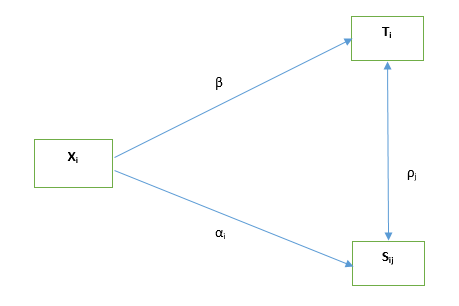
\includegraphics[scale=0.7]{modelframework.PNG}
		\caption{Model Framework}
	\end{figure}
	
	$\alpha$ and $\beta$ remains as defined above but $\rho_{S,T|Z}$ is the adjusted association.
	The model framework above was also used to depict the Quantitative Structure Transcription-Assay Relationship(QSTAR)\citep{surrogate1}.  Generally, the method involves fitting the bivariate linear regression model $(1)$ and $(2)$ which can as well be defined as;
	
	\begin{equation}\label{bivariateregression}
	\left( \begin{array}{c}
	S_{ij} \\
	T_{i}
	\end{array} \right) \sim N\left[ \left( \begin{array}{c}
	\mu_{S} + \alpha_jX_i  \\
	\mu_{T} + \beta X_i
	\end{array}
	\right), \Sigma_j \right], \ \ \Sigma_j = \left( \begin{array}{cc}
	\sigma_{SS} & \sigma_{ST}\\
	\sigma_{ST} & \sigma_{TT}
	\end{array}\right)
	\end{equation}
	
	Equation \ref{bivariateregression} above is for a case of multiple surrogates. From the $\Sigma$ matrix in $(7)$, the adjusted association\citep{surrogate1,surrogate2} can easily be computed as;
	
	\begin{equation}
	\rho_{S,T|Z} = \frac{\sigma_{ST}}{\sqrt{\sigma_{SS} \sigma_{TT} }}
	\end{equation}
	
	where $\sigma_{ST}$ is the covariance between the residuals $\epsilon_{Sj}$ and $\epsilon_{Tj}$ of $(1)$ and $(2)$, $\sigma_{SS}$ is the variance of $\epsilon_{Sj}$ and $\sigma_{TT}$ is the variance of $\epsilon_{Tj}$. This association details the relationship between S and T after adjusting for treatment effect\citep{surrogate1,surrogate2,buyseM} at the individual level. It can also be viewed as how accurately $S$ can predict $T$, accounting for $Z$\citep{surrogate3}. One can construct a confidence interval for $\rho_{S,T|Z}$ based on the Fisher $Z$ transformation\citep{surrogate1} or fit the following reduced form of (\ref{bivariateregression})
	
	\begin{equation}\label{bivariateregression2}
	\left( \begin{array}{c}
	S_{ij} \\
	T_{i}
	\end{array} \right) \sim N\left[ \left( \begin{array}{c}
	\mu_{S} + \alpha_jX_i  \\
	\mu_{T} + \beta X_i
	\end{array}
	\right), \Sigma_j \right], \ \ \Sigma_j = \left( \begin{array}{cc}
	\sigma_{SS} & 0\\
	0 & \sigma_{TT}
	\end{array}\right)
	\end{equation}
	
	to test the hypothesis $H_0: \rho_{S,T|Z} = 0$. This can be achieved via the comparison of (\ref{bivariateregression}) and (\ref{bivariateregression2}) using a likelihood ratio test\citep{surrogate1}. Outside the realm of surrogate endpoint evaluation, $\rho_{S,T|Z}$ has found other applications. Perualia-Tan et al\citep{nolen2016} used it in computing the association between a gene expression and the response of interest, after adjusting for fingerprint effect in the QSTAR modelling framework\citep{surrogate1}.\\
	
	The adjusted association as a measure of surrogacy has  some quite interesting features; it remains within the unit interval and is precisely computed in the case of large individual level replicates. It however does not have a direct extension to where either $S$ or $T$ or both are not continuous\citep{surrogate1,surrogate2,buyseM}. Moreover, $\rho_{S,T|Z}$ does not really depict the causal relationship between $Z, T$ and $Z, S$ which is of main interest in evaluating a surrogate\citep{wim2016}. This can actually be avoided with use of strong unverifiable assumptions but, this points to need for a framework that allows the association of interest to be measured, hence the causal inference approach\citep{surrogate3}. 
	
	\subsection{Causal Inference Approach (CIA)}
	As indicated in the last paragraph of the JMA subsection, there is need to establish a causal association between the treatment effect on true endpoint $(Z,T)$ and treatment effect on surrogate $(Z,S)$, especially if the data is arising from a single clinical trial\cite{wim2016}. Furthermore, the precision of the adjusted association largely depends on the individual level replications(sample size), hence establishing surrogacy with this metric using data from a single trial with few patients might not be ideal\citep{wim2016,surrogate3}.\\
	
	Assuming that there are only two treatments being evaluated(say a standard and experimental treatment in our setting) and adopting Rubin's causal inference\citep{causal1} ideology, each patient in a trial has four potential outcomes; $T_{0j}, T_{1j}, S_{0j}, S_{ij}$, assuming $Z = 0$ and $Z = 1$ for standard and experimental treatment respectively, $j$ here is a counter for patients and not surrogates as earlier used. One could compute Individual Causal Effects(ICEs)\citep{surrogate3} as; 
	
	\begin{eqnarray}
	\Delta T &=&  T_{1j} - T_{j}\\
	\Delta S &=&  S_{1j} - S_{0j}
	\end{eqnarray}
	
	Averaging ICEs across all patients in the trial gives the Expected Causal Effects(ECEs) in the trial\citep{surrogate3}. ICEs are however not identifiable from the data, since patients are randomized to take a certain treatment and not the two treatments, hence only two of the four potential outcomes are observed\citep{surrogate1,surrogate3}. However, if it is assumed that the observations from a patient is independent of other patients (Stable Unit Treatment Value Assumption, SUTVA), with $T_j$ and $S_j$ the observed true and surrogate endpoint values for patient $j$, then it follows that;
	
	\begin{eqnarray}
	T_j &=& Z_jT_{1j} + (1 - Z_j)T_{0j}\\
	S_j &=& S_jT_{1j} + (1 - Z_j)S_{0j}
	\end{eqnarray}
	
	where, $Z_j$ is the treatment group the patient $j$ is randomized to. If it is further assumed that treatment group is independent of potential outcomes(this assumption is always guaranteed in clinical trials because of randomization), i.e. $Z \perp (T_{0j}, T_{1j})$ and $Z \perp (S_{0j}, S_{1j})$, then;
	
	\begin{eqnarray}
	\beta &=& E(T_j|Z_j=1) - E(T_{j}|Z_j=0)\\
	\alpha &=& E(S_j|Z_j=1) - E(S_{j}|Z_j=0)
	\end{eqnarray}
	where $\alpha$ and $\beta$ retain the same meaning as in (1) and (2) because of the for-mentioned assumptions\citep{surrogate3,wim2016}. Furthermore, these two quantities are the expected causal effects of $Z$ on $S$ and $T$\citep{surrogate1} and are estimable from the observed data.\\ 
	
	Let's assume that the set of potential outcomes is normally distributed, i.e. $Y = (T_{0j},T_{1j},S_{0j},S_{1j}) \sim N(\mu, \Sigma)$,\ \  $\mu = (\mu_{0j},\mu_{1j},\mu_{0j},\mu_{1j})$ and $\Sigma = \left( \begin{array}{cccc}
	\sigma_{T_0 T_0} & \sigma_{T_0 T_1} & \sigma_{T_0 S_0} & \sigma_{T_0 S_1}\\
	\sigma_{T_0 T_1} & \sigma_{T_1 T_1} & \sigma_{T_1 S_0} & \sigma_{T_1 S_1}\\
	\sigma_{T_0 S_0} & \sigma_{T_1 S_0} & \sigma_{S_0 S_0} & \sigma_{S_0 S_1}\\
	\sigma_{T_0 S_1} & \sigma_{T_1 S_1} & \sigma_{SS_0 S_1} & \sigma_{S_1 S_1}
	\end{array} \right)$, it then follows that the vector of ICEs can be written as $AY$, where $A = (1, -1, 1, -1)$. It further follows that $AY \sim N(A \mu, A \Sigma A')$, where $A \mu = (\beta, \alpha)$\citep{surrogate1}. 
	
	This implies that a confidence interval cannot be estimated for $\rho_{ICA}$ since the quantity in itself is estimated via several guess of plausible values.
	
	\subsection{Evaluating Use of Multiple Surrogates}
	
	\subsection{Softwares and Tools}
	The packages \emph{Surrogate}\citep{R2} and \emph{nlme}\citep{R3} in R 3.4.0\citep{R} are the major software tools employed in analyzing the data used for this thesis. Also, the packages \emph{exactRankTests}\citep{R4} and \emph{multtest}\citep{R5} were used for non-parametric testing of treatment effect and correcting for multiplicity respectively.
	
	\section{Data Analysis}
	This section present the results obtained by applying the Joint Modelling and Causal Inference surrogate endpoint evaluation approach to the dataset described in the first section of this report. First, an exploration of the association between each surrogate and the true endpoint is presented, then the treatment effect on insulin sensitivity as well as the surrogates is carried out using both parametric (paired t-test\citep{DNAmicroarray}) as well as non-parametric test (Wilcoxon rank sum test\citep{DNAmicroarray}). The non-parametric alternative to the paired t-test was considered because of concerns about the number of individuals involved in the study. Also, focus will be on log of the surrogates since they are primarily difference in counts.
	
	\subsection{Exploratory Analysis}
	A scatter plot of insulin sensitivity $(T)$ against bacteria counts $(S)$, with each point coloured based on treatment received $(Z)$ is used to explore the association between these variables. This is done using both the raw counts and log of counts for each bacteria cell, however explanations will be focused on log counts rather than the counts themselves.
	
	\begin{figure}[H]
		\begin{minipage}{0.5\textwidth}
			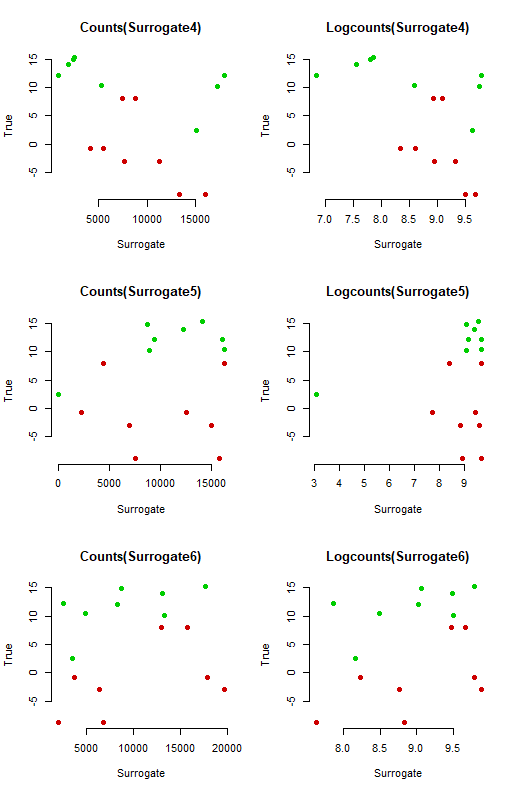
\includegraphics[scale=0.5]{exploration-2.png}\\(a)
			%\end{figure}
		\end{minipage}
		\begin{minipage}{0.5\textwidth}
			%\begin{figure}[H]
			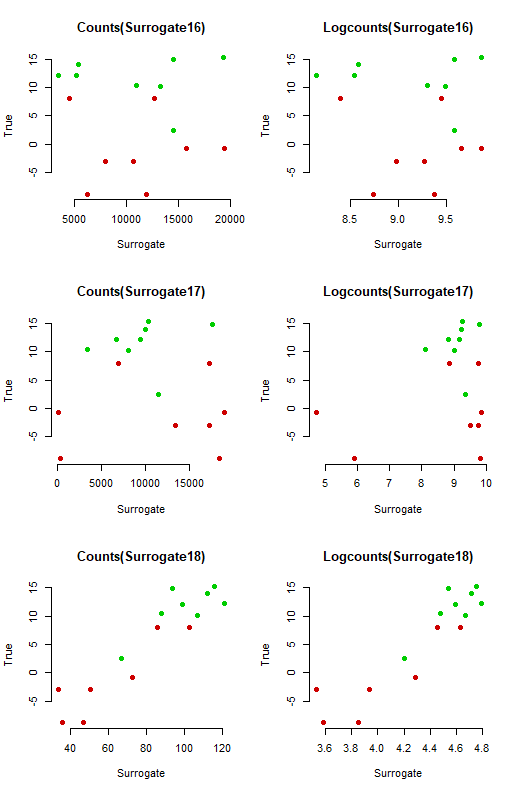
\includegraphics[scale=0.5]{exploration-6.png}\\(b)
		\end{minipage}
		\caption{\small \textit{Scatterplots of insulin sensitivity against each surrogate coloured by treatment received. Red=autologous gut microbiota infusion (control treatment), green=allogenic gut microbiota infusion (experimental treatment)}}
	\end{figure}
	A look at the grouping of colours from the y-axis shows the treatment effect on insulin sensitivity, the colour grouping along the x-axis along the would indicate treatment effect on the surrogate, while the arrangement of the points across and within the colour groups gives an idea of the association between insulin sensitivity and the surrogates.\\
	
	Generally in all the figures (2,3 and the rest in appendix), one could observe that the green points (experimental treatment) is above the red ones (control treatment) indicating a treatment effect on insulin sensitivity. In terms of the surrogates, the plots suggests a treatment effect on surrogates; 18 (figure 2b), 29 and 13 (figure 3a and b). 
	
	\begin{figure}[H]
		\begin{minipage}{0.5\textwidth}
			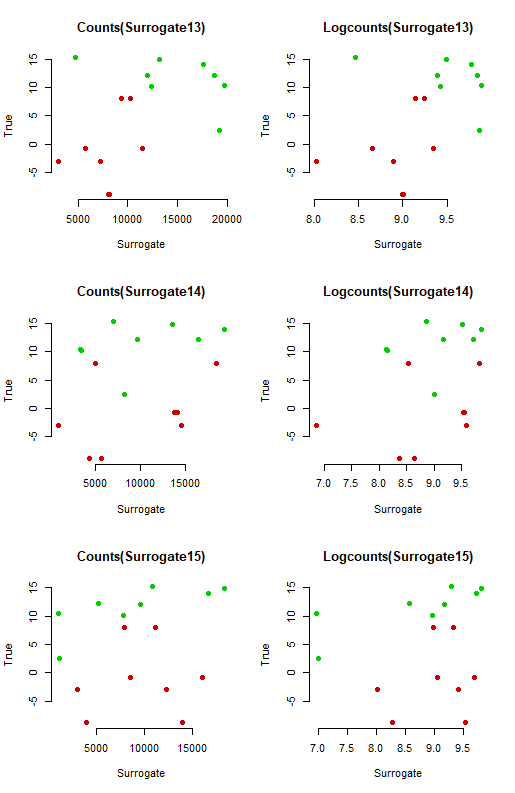
\includegraphics[scale=0.5]{exploration-5.png}\\(a)
			%\end{figure}
		\end{minipage}
		\begin{minipage}{0.5\textwidth}
			%\begin{figure}[H]
			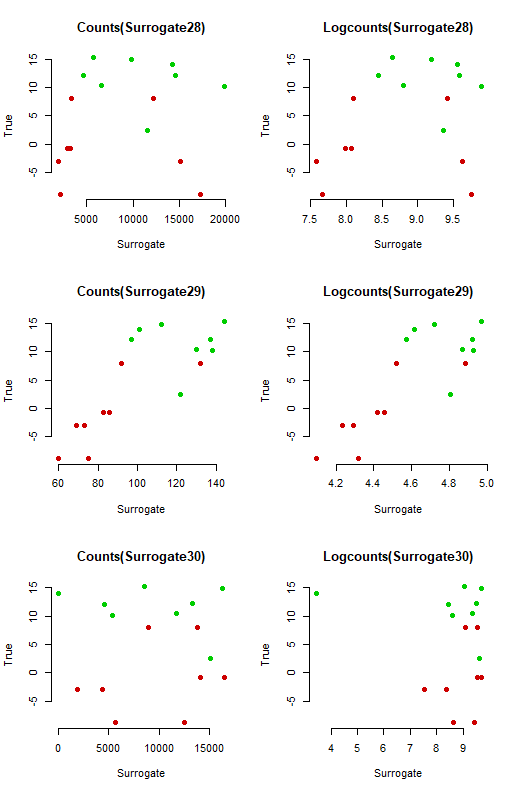
\includegraphics[scale=0.5]{exploration-10.png}\\(b)
		\end{minipage}
		\caption{\small \textit{Scatterplots of insulin sensitivity against each surrogate coloured by treatment received. Red=autologous gut microbiota infusion (control treatment), green=allogenic gut microbiota infusion (experimental treatment)}}
	\end{figure}
	In terms of the association, surrogates 18 appears interesting since a linear association is visible between both the red (control) and green (experimental) points. This indicates the likelihood of a high adjusted association between this surrogate and the true endpoint. This observation is also consistent for surrogate 29, however the association appears stronger within the control group than within the experimental group. Furthermore, surrogate 4 appears to have a negative association with insulin sensitivity in both treatment groups. These observations remain consistent with those that can be deduced from table \ref{correlationtable}. A careful look at surrogate 29 in table \ref{correlationtable} reveals high $\rho_{UN}$ (0.82) but this mainly driven by the high $\rho_0$. Furthermore, it is also important to note that $\rho_0$ and $\rho_1$ are in different directions.
	
	\begin{table}[H]
		\centering
		\begin{tabular}{ccc}
			\hline
			$S$ & $\rho_{0}$ & $\rho_{1}$ \\ 
			\hline
			1 & 0.01 & -0.24 \\ 
			2 & 0.32 & -0.01 \\ 
			3 & 0.20 & -0.38 \\ 
			4 & -0.49 & -0.59 \\ 
			5 & -0.16 & 0.88 \\ 
			6 & 0.57 & 0.56 \\ 
			7 & 0.06 & -0.32 \\ 
			8 & -0.52 & 0.37 \\ 
			9 & 0.19 & 0.01 \\ 
			10 & -0.48 & 0.18 \\ 
			11 & -0.57 & 0.70 \\ 
			12 & -0.27 & 0.09 \\ 
			13 & 0.29 & -0.50 \\ 
			14 & 0.32 & 0.32 \\ 
			15 & 0.20 & 0.79 \\
			\hline
		\end{tabular}
		\quad
		\begin{tabular}{ccc}
			\hline
			$S$ & $\rho_{0}$ & $\rho_{1}$ \\ 
			\hline
			16 & -0.10 & -0.15 \\ 
			17 & 0.21 & 0.14 \\ 
			18 & 0.84 & 0.81 \\ 
			19 & 0.00 & 0.21 \\ 
			20 & -0.51 & 0.73 \\ 
			21 & 0.12 & -0.47 \\ 
			22 & 0.43 & -0.10 \\ 
			23 & 0.06 & 0.30 \\ 
			24 & -0.10 & 0.81 \\ 
			25 & 0.18 & -0.47 \\ 
			26 & 0.39 & -0.19 \\ 
			27 & -0.44 & 0.16 \\ 
			28 & 0.02 & -0.23 \\ 
			29 & 0.85 & -0.11 \\ 
			30 & 0.28 & -0.28 \\ 
			\hline
		\end{tabular}
		\quad
		\begin{tabular}{cc}
			\hline
			$S$ & $\rho_{UN}$ \\ 
			\hline
			1 & -0.23 \\ 
			2 & -0.34 \\ 
			3 & -0.23 \\ 
			4 & -0.52 \\ 
			5 & 0.14 \\ 
			6 & 0.29 \\ 
			7 & -0.29 \\ 
			8 & 0.22 \\ 
			9 & 0.33 \\ 
			10 & -0.20 \\ 
			11 & -0.05 \\ 
			12 & -0.10 \\ 
			13 & 0.44 \\ 
			14 & 0.29 \\ 
			15 & 0.12 \\ 
			\hline
		\end{tabular}
		\quad
		\begin{tabular}{cc}
			\hline
			$S$ & $\rho_{UN}$ \\
			\hline
			16 & -0.13 \\ 
			17 & 0.27 \\ 
			18 & 0.90 \\ 
			19 & -0.22 \\ 
			20 & -0.14 \\ 
			21 & -0.03 \\ 
			22 & 0.29 \\ 
			23 & 0.17 \\ 
			24 & -0.18 \\ 
			25 & -0.01 \\ 
			26 & 0.31 \\ 
			27 & 0.10 \\ 
			28 & 0.31 \\ 
			29 & 0.82 \\ 
			30 & -0.18 \\ 
			\hline
		\end{tabular}
		\caption{\emph{Correlations between each surrogate(S) and insulin sensitivity(T). S=Surrogates, $\rho_0$=correlation between S and T in the control group, $\rho_1$=correlation between S and T in the experimental group and $\rho_{UN}$=correlation between S and T without paying attention to treatment group.}}\label{correlationtable}
	\end{table}
	
	This implies that the association between insulin sensitivity and surrogate 29 is different based on the treatment group. The association between surrogate 4 and insulin sensitivity is consistent in both treatment groups (see $\rho_0$ and $\rho_1$ in table,  \ref{correlationtable}), this observation is also consistent for surrogate 18 and 6.
	
	\subsection{Estimation of Treatment Effects}
	In estimating treatment effects, the following null hypothesis is of interest for insulin sensitivity;
	$$ H_0: \mu_{0} = \mu_{1}$$
	where $\mu_{0}$ is the average insulin sensitivity value for the patients administered the control treatment and $\mu_{1}$ the average insulin sensitivity value for patients administered the experimental treatment. The same hypothesis is of interest for each surrogate but because there are several surrogates, the index j will be added to the subscript 0 and 1 in the previous hypothesis. Hence the null;
	
	$$ H_0: \mu_{0j} = \mu_{1j}, \ \ \ j=1, 2, \ldots, 30$$
	is of interest. Here, $\mu_{0j}$ is the average difference in count for surrogate $j$ from patients administered the control treatment, while $\mu_{1j}$ is the average difference in count for surrogate $j$ from patients administered the experimental treatment. The second hypothesis testing involves 30 different hypothesis, hence the need for multiplicity correction. The Benjamini-Hockberg (BH) approach\citep{DNAmicroarray} to correcting False Discovery Rate (FDR) was employed. Also, these null hypotheses are tested against their two-sided alternatives.
	
	\begin{table}[H]
		\centering
		\begin{tabular}{cccc}
			\hline
			Type & MeanDifference & LowerCI & UpperCI\\
			\hline
			t & 12.57 & 6.68 & 18.47\\
			W & 13.23 & 5.45 & 18.96\\
			\hline
		\end{tabular}
		\caption{\emph{Results of student-t (t) and Wilcoxon (W) test for difference in means. MeanDifference is estimated as $\mu_{1} - \mu_{0}$ for t and $R_{1} - R_{2}$ for W. $R_1$ is sum of ranks for experimental group while $R_0$ is the sum of ranks for the control group.}}\label{Tresults}
	\end{table}
	Results from table \ref{Tresults} showed that the experimental group had a higher average insulin sensitivity compared to the control group. The resulting confidence interval for the difference in means also did not contain 0, hence it can be concluded that there is a significant difference in means of the experimental and control group. Due to concerns about the sample size (as indicated earlier), the same hypothesis was also tested in a non-parametric fashion using the Wilcoxon ranksum test. Similar conclusions were derived from this test as well, however the confidence interval for the treatment effect was larger compared to the student-t.\\
	
	In terms of treatment effect on surrogates, there is a significant treatment effect (at 5\% level of significance) on surrogates 29, 18 and 13 when student-t is applied, however surrogate is added to the list when Wilcoxon ranksum test is used (see raw p-value column in table \ref{surrogate treatment effects}). When multiplicity is adjusted for, none of the surrogates have a significant treatment effect in both tests.
	
	\begin{figure}[H]
		\begin{minipage}{0.5\textwidth}
			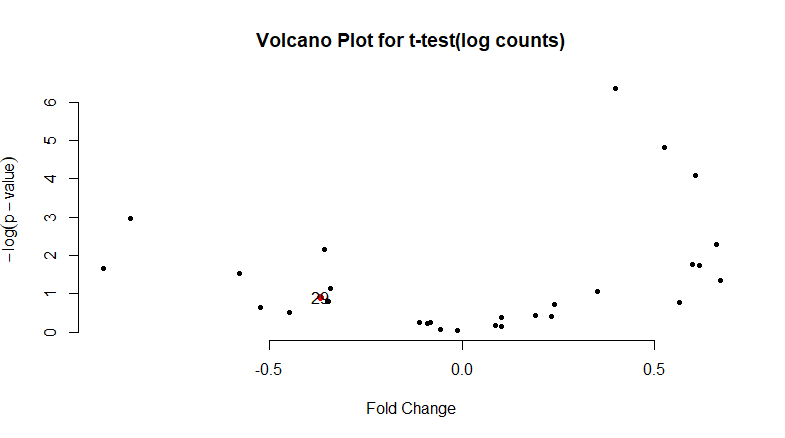
\includegraphics[scale=0.45]{t-testvolcano_plot_logcounts.png}\\(a)
			%\end{figure}
		\end{minipage}
		\begin{minipage}{0.5\textwidth}
			%\begin{figure}[H]
			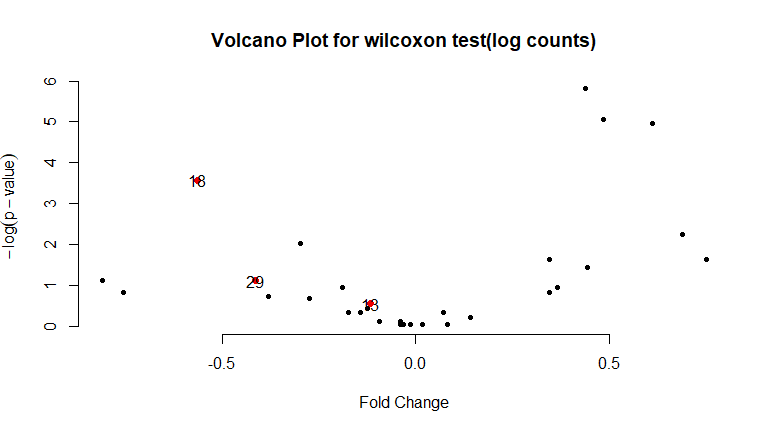
\includegraphics[scale=0.45]{wilcox_volcano_plot_logcounts.png}\\(b)
		\end{minipage}
		\caption{\small \textit{Volcano plots of fold change against -log(raw p-value) for both t-test and Wilcoxon. Fold change in t-test is computed as difference in means while it is computed as difference in ranks for Wilcoxon ranksum test. Surrogates with adjusted p-value $<$ 0.1 is in red with the surrogate number on it.}}\label{volcanoplots}
	\end{figure}
	Figures \ref{volcanoplots} (a) and (b) also showed that surrogates 29 have an adjusted p-value $<$ 10\% in both student-t and Wilcoxon test while surrogates 18 and 13 also have adjusted p-values $<$ 10\%. Therefore, in terms of treatment effects, surrogates 29, 18 and 13 could be explored for treatment effects, however this is not certain because they aren't validated surrogates and a relationship has not been established between the effect of treatment on insulin sensitivity and the effect of treatment on these surrogates. This is the topic of the following subsections.
	
	\subsection{Univariate Surrogate Evaluation}
	In this part of the report, results obtained from applying the two methods discussed in the previous section to each surrogate is presented and discussed.
	
	\subsubsection{Joint Modelling Results}
	For each surrogate, model (\ref{bivariateregression}) and (\ref{bivariateregression2}) is fitted and compared using a likelihood ratio test, the adjusted association $(\rho_{S,T|Z})$ is computed as described previously and the Fisher Z approach is used to construct a confidence interval for the adjusted association. Of interest in comparison of these 2 models is the null hypothesis,
	
	$$H_0: \rho_{S,T | Z} = 0$$
	against its two sided alternative. Since there are 30 surrogates, it implies that a multiplicity issue arises again, hence the BH procedure to controlling FDR is also employed here.
	Also, treatment effect on each surrogate and insulin sensitivity is evaluated.
	
	\begin{table}[H]
		\centering
		\resizebox{3in}{!}{ %
			\begin{tabular}{ccccccc}
				\hline
				S & $\rho_{S,T|Z}$ & $S_{Trt}$ & $PV_S$ & $BH_S$ & $PV_{\rho_{S,T|Z}}$ & $BH_{\rho_{S,T|Z}}$ \\ 
				\hline
				18 & 0.83 & 0.52 & 0.00 & 0.04 & 0.00 & 0.00 \\ 
				29 & 0.57 & 0.40 & 0.00 & 0.01 & 0.01 & 0.13 \\ 
				6 & 0.56 & -0.11 & 0.77 & 0.92 & 0.01 & 0.13 \\ 
				15 & 0.46 & -0.35 & 0.44 & 0.80 & 0.05 & 0.36 \\ 
				4 & -0.44 & -0.58 & 0.19 & 0.58 & 0.06 & 0.36 \\ 
				5 & 0.41 & -0.45 & 0.60 & 0.88 & 0.09 & 0.44 \\ 
				14 & 0.32 & 0.19 & 0.65 & 0.88 & 0.19 & 0.74 \\ 
				27 & -0.31 & 0.62 & 0.16 & 0.58 & 0.20 & 0.74 \\ 
				24 & 0.25 & -0.36 & 0.10 & 0.52 & 0.30 & 0.82 \\ 
				10 & -0.24 & -0.09 & 0.80 & 0.92 & 0.34 & 0.82 \\ 
				22 & 0.23 & 0.24 & 0.48 & 0.80 & 0.35 & 0.82 \\ 
				11 & -0.22 & 0.10 & 0.67 & 0.88 & 0.38 & 0.82 \\ 
				17 & 0.19 & 0.56 & 0.45 & 0.80 & 0.44 & 0.82 \\ 
				20 & -0.19 & -0.06 & 0.93 & 0.96 & 0.45 & 0.82 \\ 
				26 & 0.19 & 0.35 & 0.34 & 0.78 & 0.45 & 0.82 \\
				\hline
			\end{tabular} %
		}
		\quad
		\resizebox{3in}{!}{ %
			\begin{tabular}{ccccccc}
				\hline
				S & $\rho_{S,T|Z}$ & $S_{Trt}$ & $PV_S$ & $BH_S$ & $PV_{\rho_{S,T|Z}}$ & $BH_{\rho_{S,T|Z}}$ \\ 
				\hline
				9 & 0.15 & 0.67 & 0.24 & 0.65 & 0.55 & 0.82 \\ 
				12 & -0.14 & -0.01 & 0.96 & 0.96 & 0.58 & 0.82 \\ 
				7 & -0.13 & -0.34 & 0.31 & 0.77 & 0.59 & 0.82 \\ 
				23 & 0.12 & 0.23 & 0.66 & 0.88 & 0.62 & 0.82 \\ 
				3 & -0.12 & -0.35 & 0.43 & 0.80 & 0.64 & 0.82 \\ 
				16 & -0.12 & -0.08 & 0.77 & 0.92 & 0.64 & 0.82 \\ 
				21 & -0.11 & 0.10 & 0.86 & 0.92 & 0.65 & 0.82 \\ 
				2 & 0.10 & -0.86 & 0.03 & 0.26 & 0.69 & 0.82 \\ 
				8 & -0.10 & 0.60 & 0.16 & 0.58 & 0.70 & 0.82 \\ 
				19 & 0.10 & -0.93 & 0.17 & 0.58 & 0.70 & 0.82 \\ 
				1 & -0.09 & -0.37 & 0.40 & 0.80 & 0.71 & 0.82 \\ 
				25 & -0.08 & 0.09 & 0.85 & 0.92 & 0.75 & 0.84 \\ 
				30 & -0.06 & -0.52 & 0.51 & 0.80 & 0.80 & 0.86 \\ 
				28 & -0.05 & 0.66 & 0.08 & 0.51 & 0.84 & 0.87 \\ 
				13 & -0.04 & 0.61 & 0.01 & 0.11 & 0.88 & 0.88 \\
				\hline
			\end{tabular}  %
		}
		\caption{\emph{Table showing $\rho_{S,T|Z}$, treatment effect on surrogate as well as raw and adjusted p-values for these quantities, ordered by absolute value of $\rho_{S,T|Z}$. $S_{trt}$=treatment effect on surrogate, $PV_S,PV_{\rho_{S,T|Z}}$=raw p-values for surrogate treatment effect and $\rho_{S,T|Z}$, $BH_{S},BH_{\rho_{S,T|Z}}$=adjusted p-values for surrogate treatment effect and $\rho_{S,T|Z}$. }}\label{univariate adjusted association table}
	\end{table}
	
	The estimated treatment effect on insulin sensitivity ($\beta$ from the model framework) is 12.57, same as the difference in means for the two treatment groups, however there is a significant effect of treatment only on surrogate 18 and 29 after adjusting for multiplicity. In terms of adjusted association, all computed $\rho_{S,T|Z}$ is lesser than $\rho_{UN}$ since the effect of treatment has been removed before computing $\rho_{S,T|Z}$. A closer look at surrogate 29 revealed that the value of 0.82 for $\rho_{UN}$ reduced to 0.57 after adjusting for treatment, this association is even not significantly different from 0. Only surrogate 18 had an adjusted association value significantly different from 0 after adjusting for multiplicity. This implies that surrogate 18 is significantly correlated with insulin sensitivity regardless of treatment group, which makes surrogate 18 a good surrogate if conclusions were drawn based on this approach.
	
	\begin{figure}[H]
		\centering
		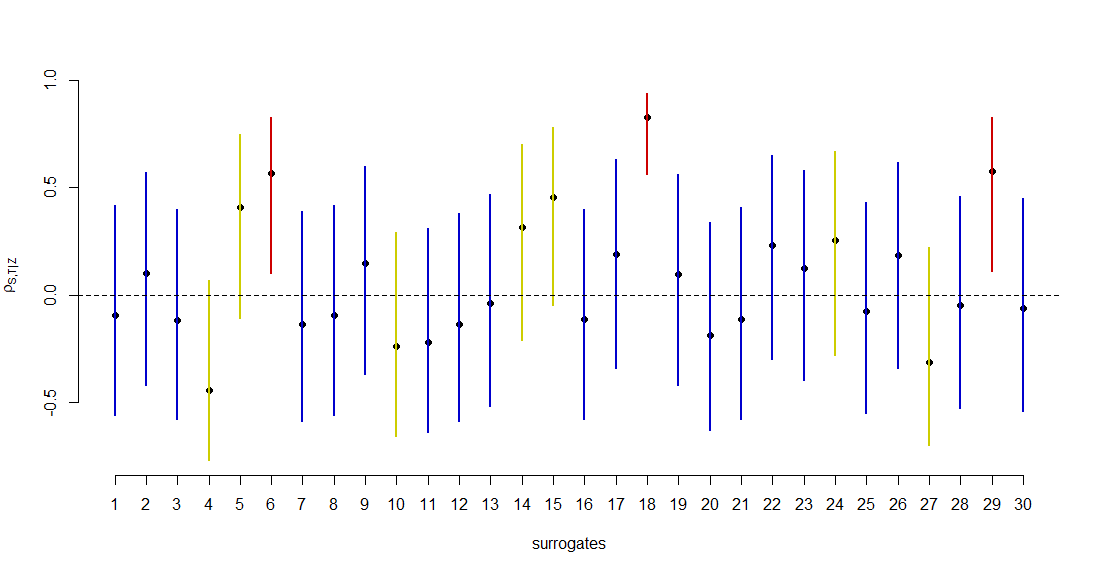
\includegraphics[scale=0.5]{adjustedassociationplot.png}
		\caption{\emph{$\rho_{S,T|Z}$(black points) for each surrogate alongside their confidence intervals. Confidence interval is coloured by order in table \ref{univariate adjusted association table}. Top 3 surrogates in red, next 7 in yellow and others in blue.}}\label{adjusted association plot}
	\end{figure}
	
	The confidence interval represents a measure of uncertainty about the estimated adjusted association. It is important to examine this in order to have an idea of the precision of the estimated adjusted association for each surrogate. A look at figure \ref{adjusted association plot} showed that $\rho_{S,T|Z}$ for surrogate 18 is estimated with high precision while $\rho_{S,T|Z}$ surrogates 6 and 29 were also estimated fairly precisely. Regarding information contained in these surrogates in relation to insulin sensitivity, surrogates 4, 10 and 27 contain somewhat different information compared to other top 10 surrogates, since the confidence interval for their $\rho_{S,T|Z}$ is in the opposite direction of others. In other words, while surrogates 4, 10 and 27 are negatively associated with insulin sensitivity after adjusting for treatment, other surrogates among the top 10 surrogates are positively associated with insulin sensitivity.
	
	\subsubsection{Causal Inference Results}
	For each surrogate, $\rho_{\Delta}$, the Individual Causal Association (ICA),  its distribution and $\delta$, the Prediction Mean Square Error (PMSE) are computed. This is done by estimating the identifiable part of $\Sigma$, convert it to a correlation matrix and filling other unidentifiable parts with plausible values between -1 and 1 as described in the methods section.  The range of $\rho_{\Delta}$ values obtained from its distribution is used as a measure of uncertainty about the computed ICA values, since a confidence interval cannot be computed for the ICA values. The distribution of $\rho_{\Delta}$ is also examined to see the general direction of computed individual causal association between each surrogate and insulin sensitivity.
	
	\begin{table}[H]
		\centering
		\begin{tabular}{cccc}
			\hline
			S & $\rho_{\Delta}$ & LR & UR \\ 
			\hline
			18 & 0.91 & -0.76 & 1.00 \\ 
			6 & 0.84 & -0.96 & 1.00 \\ 
			15 & 0.83 & -0.91 & 0.93 \\ 
			4 & -0.79 & -1.00 & 0.97 \\ 
			17 & 0.74 & -1.00 & 1.00 \\ 
			19 & 0.70 & -0.99 & 0.99 \\ 
			24 & 0.69 & -0.85 & 0.86 \\ 
			29 & 0.67 & -0.81 & 0.84 \\ 
			14 & 0.63 & -0.99 & 1.00 \\ 
			5 & 0.60 & -0.73 & 0.80 \\ 
			22 & 0.58 & -0.96 & 0.95 \\ 
			2 & 0.57 & -0.98 & 0.98 \\ 
			20 & 0.53 & -0.75 & 0.77 \\ 
			23 & 0.52 & -0.99 & 0.98 \\ 
			8 & 0.52 & -0.87 & 0.87 \\
			\hline
		\end{tabular}
		\quad
		\begin{tabular}{cccc}
			\hline
			S & $\rho_{\Delta}$ & LR & UR \\ 
			\hline
			26 & 0.51 & -0.95 & 0.95 \\ 
			11 & 0.48 & -0.75 & 0.74 \\ 
			9 & 0.48 & -0.99 & 0.99 \\ 
			3 & 0.34 & -0.94 & 0.94 \\ 
			30 & 0.33 & -0.95 & 0.95 \\ 
			28 & 0.31 & -0.99 & 0.99 \\ 
			1 & 0.30 & -0.99 & 0.98 \\ 
			12 & 0.28 & -0.97 & 0.98 \\ 
			13 & 0.17 & -0.91 & 0.90 \\ 
			7 & 0.14 & -0.98 & 0.97 \\ 
			16 & 0.13 & -0.99 & 0.99 \\ 
			25 & 0.05 & -0.93 & 0.93 \\ 
			27 & 0.05 & -0.95 & 0.95 \\ 
			10 & 0.05 & -0.93 & 0.94 \\ 
			21 & 0.03 & -0.95 & 0.94 \\ 
			\hline
		\end{tabular}
		\caption{\emph{Estimates $\rho_{\Delta}$ for each surrogates including their range ranked by absolute value of $\rho_{\Delta}$. $\rho_{\Delta}$=ICA, LR=lower range, UR=upper range}}\label{ica}
	\end{table}
	
	Results from table \ref{ica} appear to show surrogate 18 as a very good surrogate for insulin sensitivity, but the uncertainty about the computed $\rho_{\Delta}$ raises concern since its range goes from -0.76 to 1. Although the top 10 surrogates have fairly high individual causal association with insulin sensitivity, their range of computed ICA is wide enough to cast doubts about the use of these bacterias as surrogates. To really decipher the potentially good surrogates among the 30, their $\rho_{\Delta}$ distribution and the percentage of values greater than 0.5 in absolute term, out of all computed $\rho_{\Delta}$ values is examined closely. \\
	
	A look at the distribution of ICA values for surrogate 18 revealed that there is a high chance of obtaining ICA values higher than 0.5 (see figure \ref{icaplot2} a and figure \ref{icarange}), specifically this chance was  
	
	\begin{figure}[H]
		\centering
		\begin{minipage}{0.45\textwidth}
			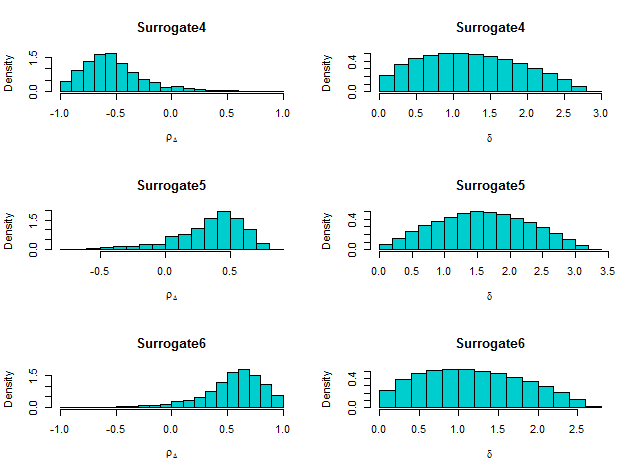
\includegraphics[scale=0.35]{icaplots2.png}\\(a)
		\end{minipage} 
		\begin{minipage}{0.45\textwidth}
			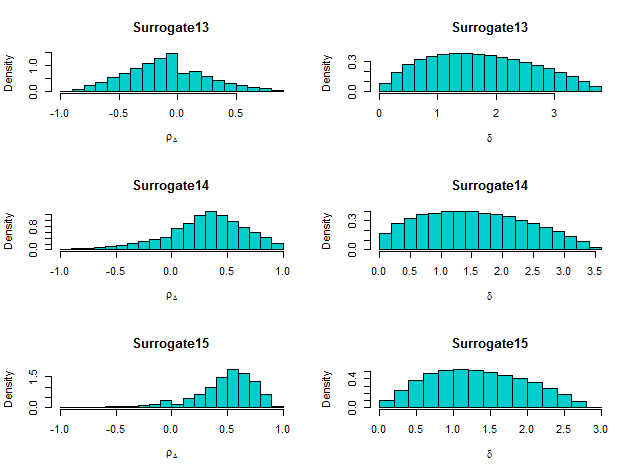
\includegraphics[scale=0.35]{icaplots5.png}\\(b)
		\end{minipage} 
		\caption{Distribution of \emph{$\rho_{\Delta}$ and $\delta$}}\label{icaplot1}
	\end{figure}
	
	%In terms of 
	
	\begin{figure}[H]
		\centering
		\begin{minipage}{0.45\textwidth}
			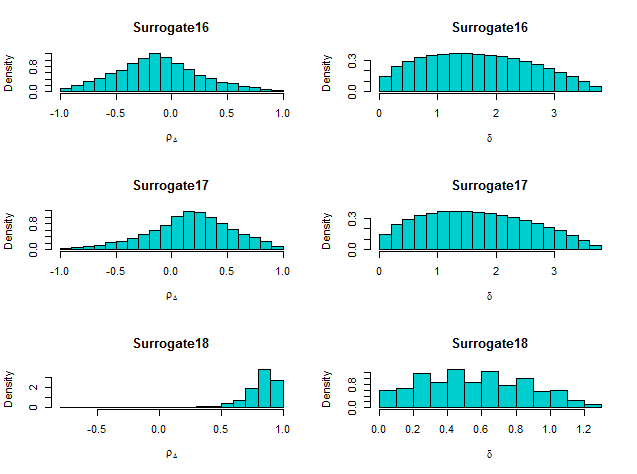
\includegraphics[scale=0.35]{icaplots6.png}\\(a)
		\end{minipage} 
		\begin{minipage}{0.45\textwidth}
			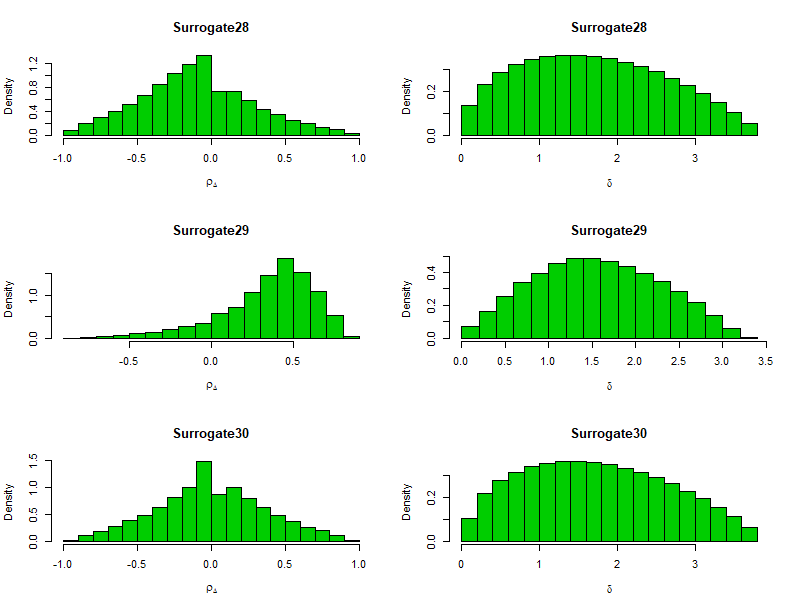
\includegraphics[scale=0.35]{icaplots10.png}\\(b)
		\end{minipage} 
		\caption{Distribution of \emph{$\rho_{\Delta}$ and $\delta$}}\label{icaplot2}
	\end{figure}
	
	\begin{figure}[H]
		\centering
		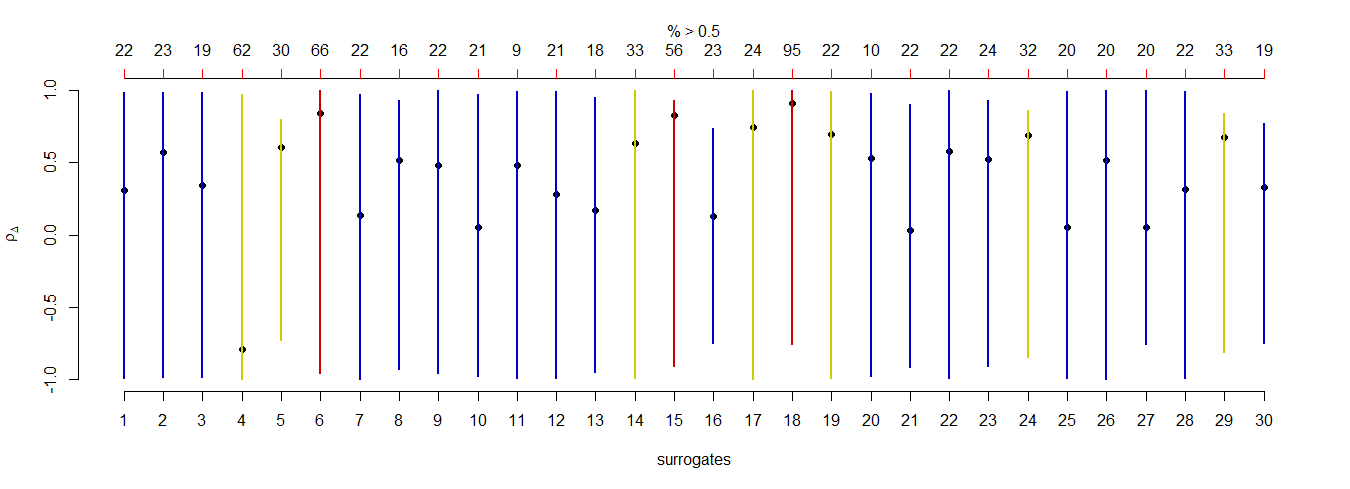
\includegraphics[scale=0.4]{icaplotRange.png}
		\caption{ \emph{$\rho_{\Delta}$ and their range including percentage greater than 0.5 in absolute value}}\label{icarange}
	\end{figure}
	
	computed to be 95\%, while this chance is 56\% and 66\% for surrogates 6 and 15. Furthermore, the skewness of the distribution of $\rho_{\Delta}$ values for these surrogates identify them as good candidates and their individual causal effects can predict the individual causal effects on insulin sensitivity with prediction error ranging from 0.5-2.5 for surrogate 15, 0.2-1.2 for surrogate 18 and 0-2.5 for surrogate 6 (see distribution of $\delta$ in figures \ref{icaplot1} and \ref{icaplot2}). For surrogate 29 which appears to be a promising surrogate judging from previous results, the chance of obtaining a $\rho_{\Delta} > 0.5$ is estimated to be 33\% while its individual causal effects will predict the individual causal effects on insulin sensitivity with errors ranging from 0-3.5. \\
	
	In terms of agreement of results obtained from joint modelling and the ones obtained here, it was observed that both methods agree on surrogate 18 been the best in terms of predicting treatment effect on insulin sensitivity from treatment effect on surrogates. Furthermore, two surrogates, 17 and 19 are found amongst the top 10 surrogates from the causal inference results and not among the top 10 from the joint modelling results, while surrogates 27 and 10 are amongst the top 10 surrogates from the joint modelling results and not among the causal inference results.\\
	
	To summarize, results obtained from surrogate by surrogate analysis, it was observed that surrogate 18 (Akkermansia) was judged the best surrogate in terms of predicting insulin sensitivity as well as treatment effect on this endpoint. While the adjusted association showed that the association between insulin sensitivity and this surrogate is precisely estimated, the range of its individual causal association covers almost the entirety of the parameter space of a correlation (-1,1). On closer inspection of the computed individual causal association, it was observed that there is a 95\% chance of obtaining individual causal association values above 0.5. It was also observed that individual causal effect on this surrogate can predict individual causal effect on insulin sensitivity with little prediction errors ranging between 0.2-1.2, this range of prediction error is the smallest when compared to other surrogates.\\ 
	
	Furthermore, it was observed that some surrogates contain information that is not captured by other surrogates, these surrogates are 4, 10 and 27. Both their adjusted association confidence interval and distribution of individual causal association values are in the opposite direction of other surrogates. Of these three surrogates, surrogate 4 appear to be most promising since its estimated individual causal association and adjusted association are negative.
	
	\subsection{Multiple Surrogates Evaluation}
	In light of the fact that some surrogates contain information not captured by other surrogates and biological evidence\citep{Vrieze, microbiome101, healthymicrobiome} that demonstrates that several element of the gut microbiota are involved in human metabolism, it is only natural to assume that a combination treatment effect on these elements would better predict  treatment effect on insulin. Furthermore, knowing that the composition of the gut microbiota vary from individual to individual but certain genes and biological pathway are maintained makes it imperative to look beyond using single elements of the microbiome as surrogates for insulin sensitivity.\\
	
	Building on results from the univariate analysis, focus will be primarily on the top 10 surrogates from both approach including the 4 surrogates not agreed on by the two methods employed. Also, since surrogate 18 is the most promising surrogate, focus will be primarily on improving this surrogate by combining it with other surrogates in the top 10. For each combination, the multivariate individual causal association and multivariate adjusted association was computed as discussed in the methods section.
	
	
	\begin{table}[H]
		\centering
		\begin{tabular}{ccccc}
			\hline
			S & $R^2_{H}$ & LR & UR & $AR^2_{H}$ \\ 
			\hline
			18,4 & 0.80 & 0.22 & 0.97 & 0.77 \\ 
			18,5 & 0.80 & 0.19 & 0.98 & 0.77 \\ 
			18,6 & 0.80 & 0.06 & 0.98 & 0.77 \\ 
			18,17 & 0.77 & 0.06 & 0.97 & 0.73 \\ 
			18,10 & 0.76 & 0.02 & 0.99 & 0.73 \\ 
			18,15 & 0.76 & 0.04 & 0.99 & 0.73 \\ 
			18,29 & 0.76 & 0.22 & 0.97 & 0.72 \\ 
			18,14 & 0.76 & 0.14 & 0.98 & 0.72 \\ 
			18,19 & 0.75 & 0.14 & 0.99 & 0.71 \\ 
			18,27 & 0.75 & 0.05 & 0.97 & 0.71 \\ 
			18,24 & 0.73 & 0.07 & 0.99 & 0.68 \\
			\hline
			(a)\\
		\end{tabular} 
		\quad
		\begin{tabular}{ccccc}
			\hline
			S & $\gamma^2_{\Delta}$ & LCL & UCL & $A\gamma^2_{\Delta}$ \\ 
			\hline
			18,4 & 0.75 & 0.52 & 0.99 & 0.71 \\ 
			18,6 & 0.75 & 0.52 & 0.99 & 0.71\\ 
			18,10 & 0.73 & 0.47 & 0.98 & 0.68\\ 
			18,5 & 0.71 & 0.45 & 0.98 & 0.67\\ 
			18,19 & 0.71 & 0.44 & 0.98 & 0.66\\ 
			18,14 & 0.70 & 0.43 & 0.97 & 0.66\\ 
			18,29 & 0.70 & 0.43 & 0.97 & 0.66\\ 
			18,17 & 0.70 & 0.43 & 0.97 & 0.66\\ 
			18,27 & 0.69 & 0.41 & 0.97 & 0.65\\ 
			18,15 & 0.69 & 0.40 & 0.97 & 0.64\\ 
			18,24 & 0.69 & 0.40 & 0.97 & 0.64\\  
			\hline
			(b)\\
		\end{tabular}
		\caption{\emph{Multivariate Individual Causal Association ($R^2_{H}$), its range, Adjusted Multivariate Individual Causal Association ($AR^2_{H}$), Multivariate Adjusted Association ($\gamma^2_{\Delta}$), its confidence interval and Adjusted Multivariate Adjusted Association ($A\gamma^2_{\Delta}$). Both tables are ordered by $R^2_{H}$ and $\gamma^2_{\Delta}$ }}\label{bivariate surrogates}
	\end{table}
	
	Results of the exercise is presented in table \ref{bivariate surrogates} and figure \ref{bivariatesurrogateplots}. The (a) part of both figure and table contain results obtained from the causal inference approach, while the (b) part contain results from the joint modelling approach.
	
	\begin{figure}[H]
		\begin{minipage}{0.5\textwidth}
			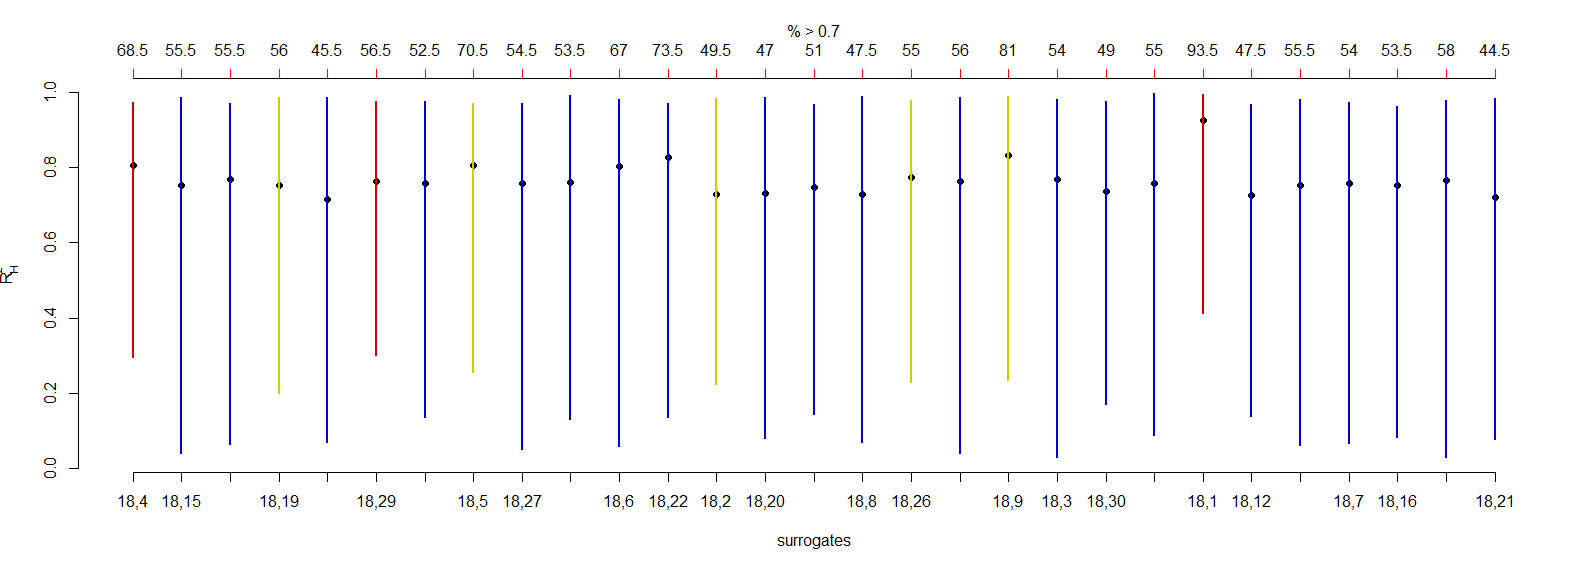
\includegraphics[scale=0.34]{bivariateSurrogateResultsMICA.png}\\(a)
			%\end{figure}
		\end{minipage}
		\begin{minipage}{0.5\textwidth}
			%\begin{figure}[H]
			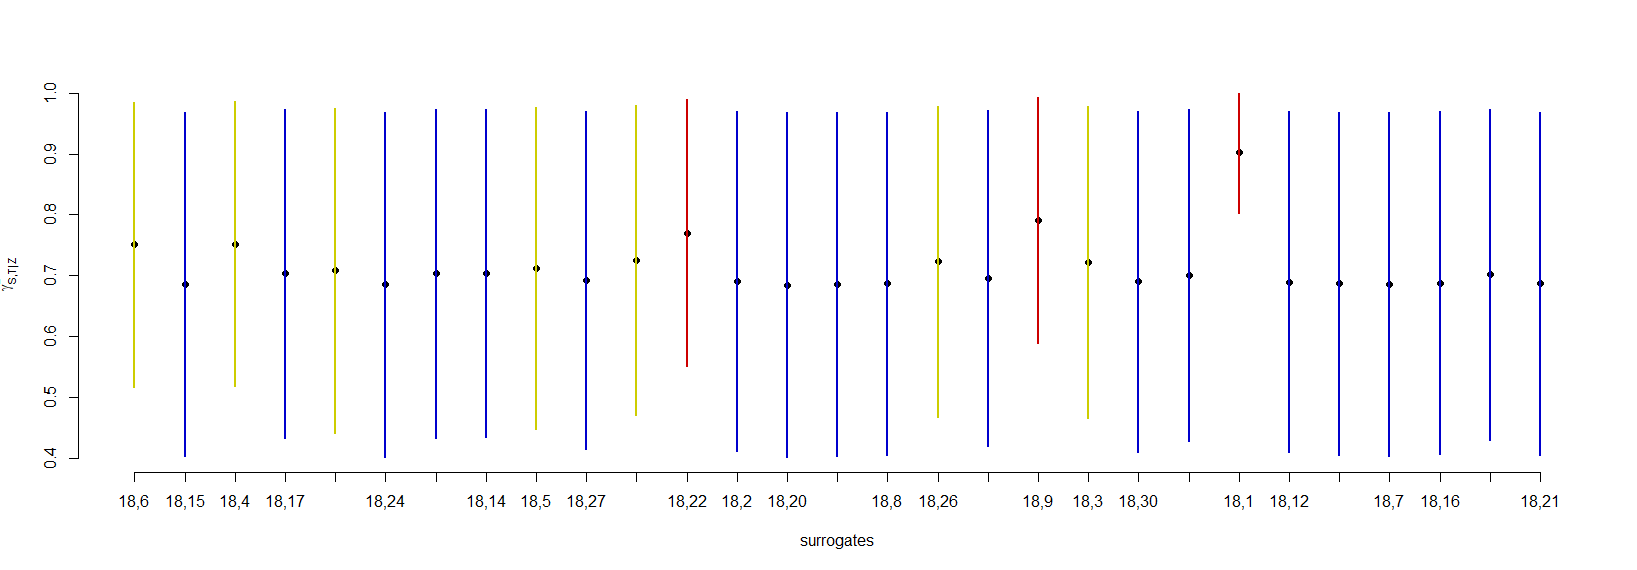
\includegraphics[scale=0.34]{bivariateSurrogateResultsMAA.png}\\(b)
		\end{minipage}
		\caption{\emph{Computed $R^2_{H}$, its range and $\gamma^2_{\Delta}$ and its confidence interval with top surrogates in red.} }\label{bivariatesurrogateplots}
	\end{figure}
	
	To properly digest these results, it is important to see if any of these surrogates improves surrogate 18, and more importantly is to check if any of the surrogates add some information to that already contained in surrogate 18. This evaluation is done by comparing results on surrogate 18 alongside those obtained here. To enable comparison on the same footing,  $\rho_{S,T|Z}^2$ for surrogate 18 is  compared with $\rho_{\Delta}$ obtained from the bivariate results. Also, the length of the range from the univariate and bivariate result are compared after the Fisher Z and logit transformation has been applied respectively. These transformations will move the range of values from $[-1,1]$ and $[0,1]$ to $[-\infty,\infty]$, thereby allowing the comparison of the range.\\
	
	The individual causal association for surrogate 18 was computed to be 
	
	
	
	%\subsubsection{Multivariate Joint Modelling Results}
	
	%\subsubsection{Multivariate Causal Inference Results}
	
	\section{Discussion \& Conclusion}
	
	
	
	\bibliography{references}
	%\printbibliography
	
	\section*{Appendix}
	\subsection*{Extra Plots}
	\subsubsection*{Exploratory Plots}
	\begin{figure}[H]
		\begin{minipage}{0.5\textwidth}
			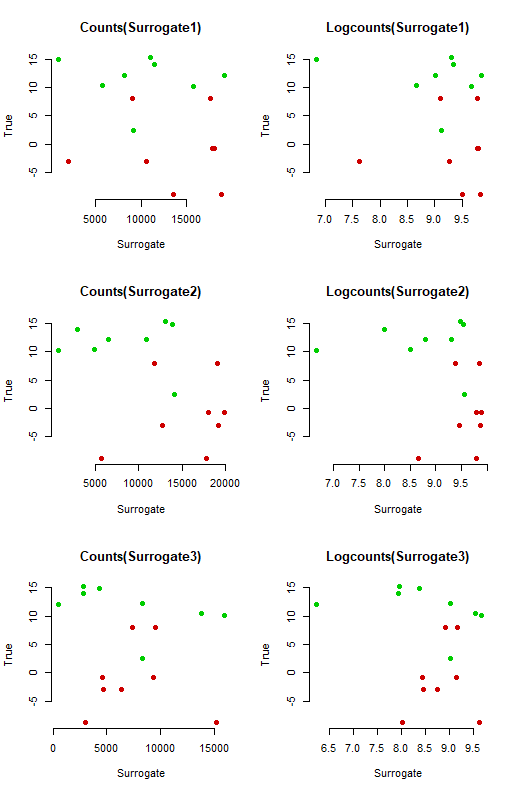
\includegraphics[scale=0.45]{exploration-1.png}
			%\end{figure}
		\end{minipage}
		\begin{minipage}{0.5\textwidth}
			%\begin{figure}[H]
			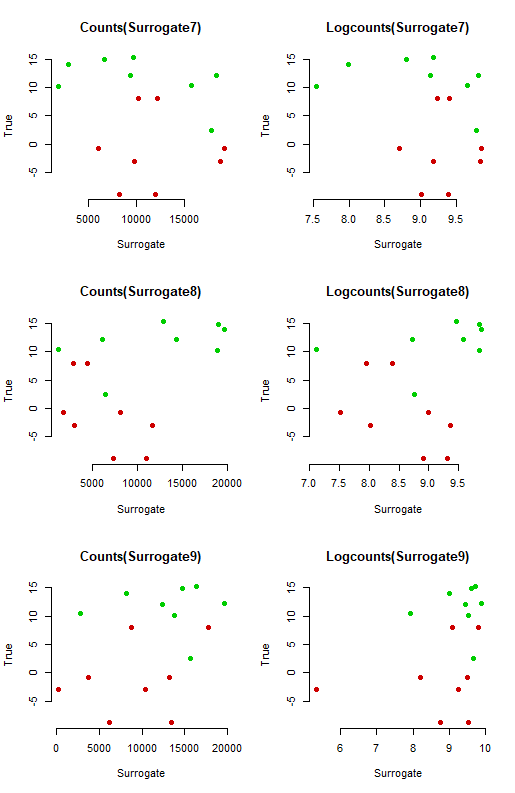
\includegraphics[scale=0.45]{exploration-3.png}
		\end{minipage}
	\end{figure}
	
	\begin{figure}[H]
		\begin{minipage}{0.5\textwidth}
			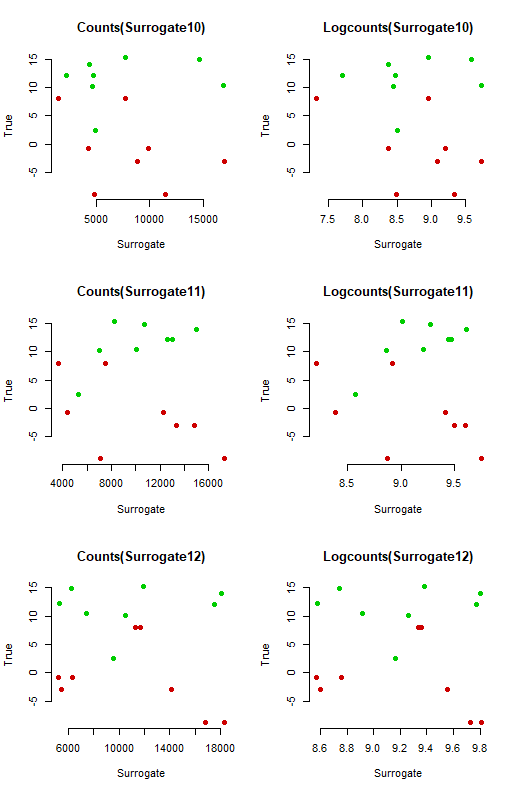
\includegraphics[scale=0.45]{exploration-4.png}
			%\end{figure}
		\end{minipage}
		\begin{minipage}{0.5\textwidth}
			%\begin{figure}[H]
			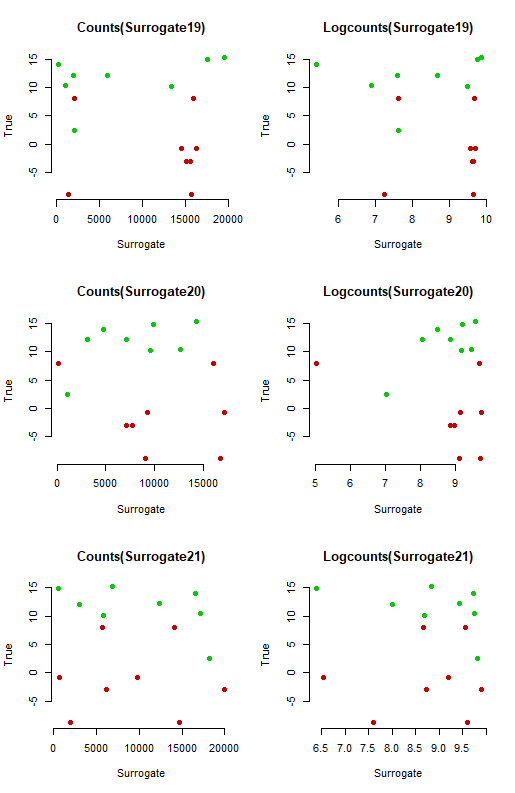
\includegraphics[scale=0.45]{exploration-7.png}
		\end{minipage}
	\end{figure}
	
	\begin{figure}[H]
		\begin{minipage}{0.5\textwidth}
			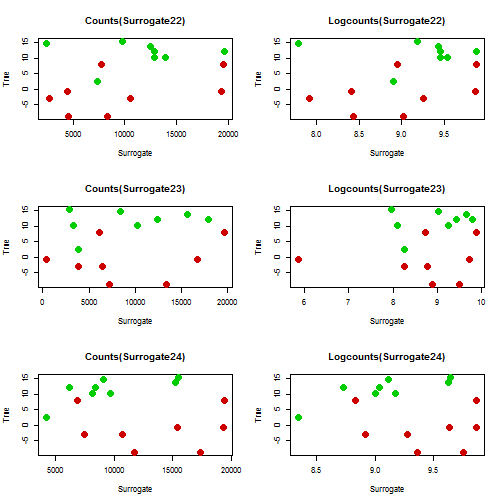
\includegraphics[scale=0.35]{exploration-8.png}
			%\end{figure}
		\end{minipage}
		\begin{minipage}{0.5\textwidth}
			%\begin{figure}[H]
			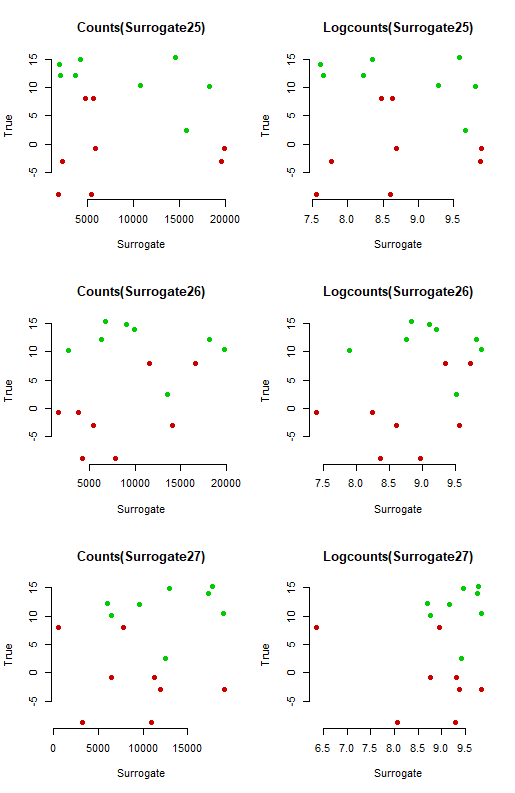
\includegraphics[scale=0.35]{exploration-9.png}
		\end{minipage}
	\end{figure}
	
	\subsubsection*{$\rho_{\Delta}$ and $\delta$ Distribution}
	\begin{figure}[H]
		\centering
		\begin{minipage}{0.45\textwidth}
			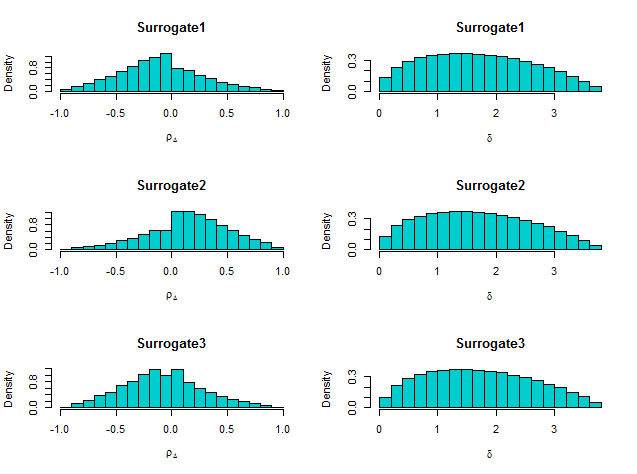
\includegraphics[scale=0.35]{icaplots1.png}\\(a)
		\end{minipage} 
		\begin{minipage}{0.45\textwidth}
			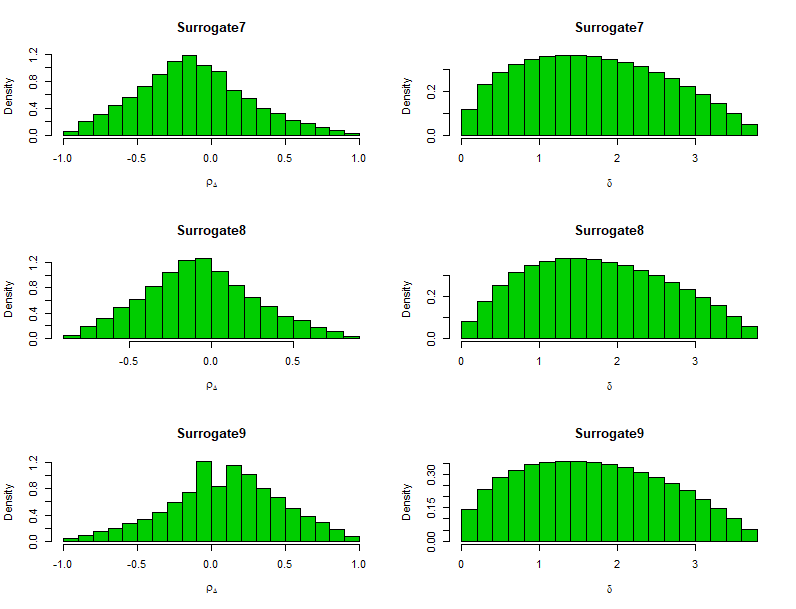
\includegraphics[scale=0.35]{icaplots3.png}\\(b)
		\end{minipage} 
		%\caption{Distribution of \emph{$\rho_{\Delta}$ and $\delta$}}
	\end{figure}
	
	\begin{figure}[H]
		\centering
		\begin{minipage}{0.45\textwidth}
			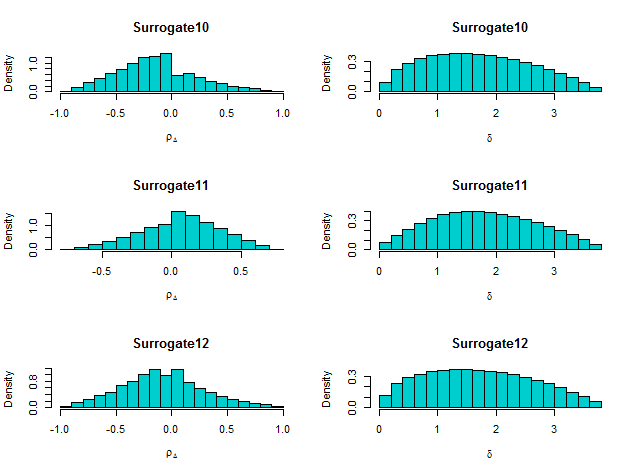
\includegraphics[scale=0.35]{icaplots4.png}\\(a)
		\end{minipage} 
		\begin{minipage}{0.45\textwidth}
			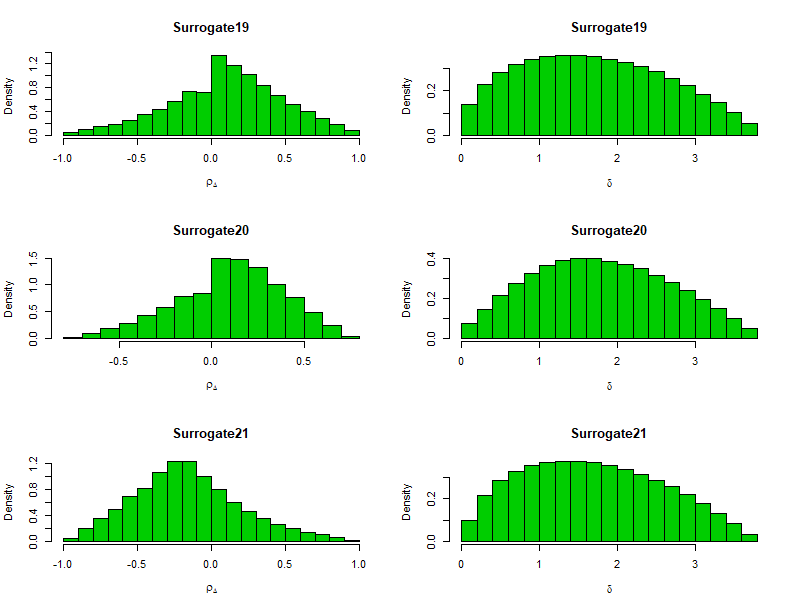
\includegraphics[scale=0.35]{icaplots7.png}\\(b)
		\end{minipage} 
		%\caption{Distribution of \emph{$\rho_{\Delta}$ and $\delta$}}
	\end{figure}
	
	\begin{figure}[H]
		\centering
		\begin{minipage}{0.45\textwidth}
			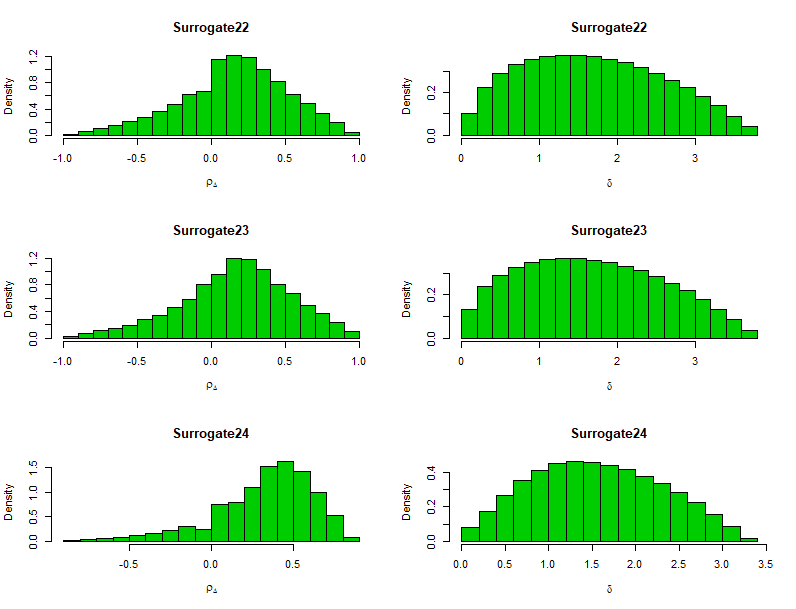
\includegraphics[scale=0.35]{icaplots8.png}\\(a)
		\end{minipage} 
		\begin{minipage}{0.45\textwidth}
			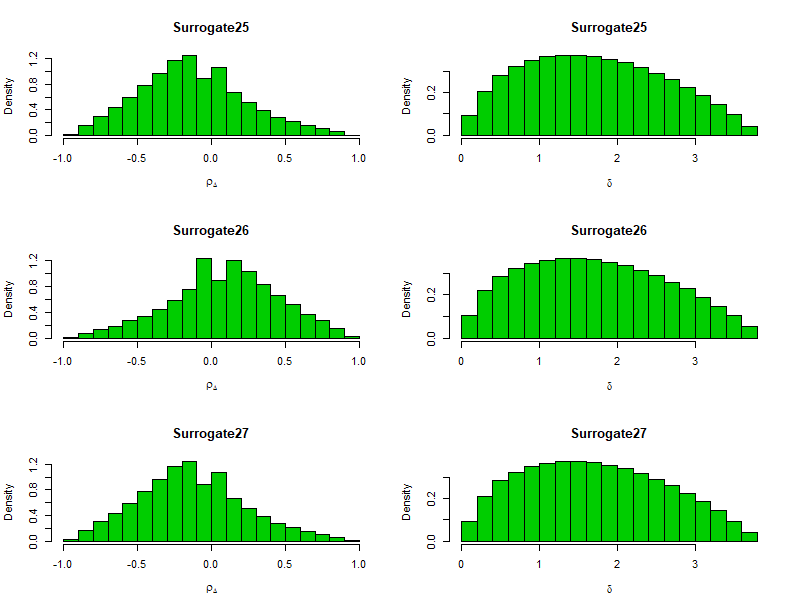
\includegraphics[scale=0.35]{icaplots9.png}\\(b)
		\end{minipage} 
		%\caption{Distribution of \emph{$\rho_{\Delta}$ and $\delta$}}
	\end{figure}
	
	\subsection*{Extra Tables}
	
	\subsubsection*{Surrogates}
	\begin{table}[H]
		\centering
		\begin{tabular}{rl}
			\hline
			S & Full Names \\ 
			\hline
			1 & Brachyspira \\ 
			2 & Lachnospira.pectinoschiza.et.rel. \\ 
			3 & Clostridium.felsineum.et.rel. \\ 
			4 & Megamonas.hypermegale.et.rel. \\ 
			5 & Mitsuokella.multiacida.et.rel. \\ 
			6 & Alcaligenes.faecalis.et.rel. \\ 
			7 & Clostridium.thermocellum.et.rel. \\ 
			8 & Lactobacillus.salivarius.et.rel. \\ 
			9 & Collinsella \\ 
			10 & Clostridium.leptum.et.rel. \\ 
			11 & Oxalobacter.formigenes.et.rel. \\ 
			12 & Papillibacter.cinnamivorans.et.rel. \\ 
			13 & Enterobacter.aerogenes.et.rel. \\ 
			14 & Oceanospirillum \\ 
			15 & Anaerostipes.caccae.et.rel. \\
			\hline
		\end{tabular}
		\quad
		\begin{tabular}{rl}
			\hline
			S & Full Names \\ 
			\hline
			16 & Klebisiella.pneumoniae.et.rel. \\ 
			17 & Bacteroides.ovatus.et.rel. \\ 
			18 & Akkermansia \\ 
			19 & Bifidobacterium \\ 
			20 & Lactococcus \\ 
			21 & Faecalibacterium.prausnitzii.et.rel. \\ 
			22 & Corynebacterium \\ 
			23 & Micrococcaceae \\ 
			24 & Helicobacter \\ 
			25 & Lactobacillus.catenaformis.et.rel. \\ 
			26 & Coprococcus.eutactus.et.rel. \\ 
			27 & Clostridium.difficile.et.rel. \\ 
			28 & Clostridium.nexile.et.rel. \\ 
			29 & Novosphingobium \\ 
			30 & Anaerotruncus.colihominis.et.rel. \\ 
			\hline
		\end{tabular}
		\caption{\emph{Full name of each Surrogate,i.e. full names of bacteria that makes up the Gut microbiota}}
	\end{table}
	
	\subsubsection*{Raw and Adjusted p-values for Surrogates}
	\begin{table}[H]
		\centering
		\begin{tabular}{ccc}
			\hline
			S & PV(t) & BH \\ 
			\hline
			29 & 0.00 & 0.05\\ 
			18 & 0.01 & 0.12\\ 
			13 & 0.02 & 0.17 \\ 
			2 & 0.05 & 0.39\\ 
			28 & 0.10 & 0.57\\ 
			24 & 0.11 & 0.57 \\ 
			8 & 0.17 & 0.63\\ 
			27 & 0.18 & 0.63\\ 
			19 & 0.19 & 0.63\\ 
			4 & 0.21 & 0.64\\ 
			9 & 0.26 & 0.70\\ 
			7 & 0.32 & 0.80\\ 
			26 & 0.34 & 0.80\\ 
			1 & 0.40 & 0.81\\ 
			3 & 0.45 & 0.81\\ 
			\hline
		\end{tabular}
		\quad
		\begin{tabular}{ccc}
			\hline
			S & PV(t) & BH\\ 
			\hline
			15 & 0.45 & 0.81\\ 
			17 & 0.47 & 0.81\\ 
			22 & 0.49 & 0.81\\ 
			30 & 0.52 & 0.82\\ 
			5 & 0.61 & 0.88\\ 
			14 & 0.66 & 0.88\\ 
			23 & 0.66 & 0.88\\ 
			11 & 0.68 & 0.88\\ 
			6 & 0.77 & 0.92 \\ 
			16 & 0.78 & 0.92\\ 
			10 & 0.80 & 0.92\\ 
			25 & 0.85 & 0.92\\ 
			21 & 0.86 & 0.92\\ 
			20 & 0.93 & 0.96\\ 
			12 & 0.96 & 0.96\\ 
			\hline
		\end{tabular}
		\quad
		\begin{tabular}{ccc}
			\hline
			S & PV(W) & BH \\ 
			\hline
			29 & 0.00 & 0.07 \\ 
			18 & 0.01 & 0.07 \\ 
			13 & 0.01 & 0.07 \\ 
			2 & 0.03 & 0.21 \\ 
			8 & 0.10 & 0.63 \\ 
			24 & 0.13 & 0.65 \\ 
			9 & 0.19 & 0.73 \\ 
			28 & 0.19 & 0.73 \\ 
			27 & 0.23 & 0.78 \\ 
			1 & 0.33 & 0.88 \\ 
			19 & 0.33 & 0.88 \\ 
			7 & 0.38 & 0.88 \\ 
			26 & 0.38 & 0.88 \\ 
			4 & 0.44 & 0.88 \\ 
			22 & 0.44 & 0.88 \\
			\hline
		\end{tabular}
		\quad
		\begin{tabular}{ccc}
			\hline
			S & PV(W) & BH \\ 
			\hline
			17 & 0.49 & 0.89 \\ 
			20 & 0.51 & 0.89 \\ 
			3 & 0.57 & 0.96 \\ 
			10 & 0.65 & 0.96 \\ 
			5 & 0.72 & 0.96 \\ 
			6 & 0.72 & 0.96 \\ 
			15 & 0.72 & 0.96 \\ 
			21 & 0.80 & 0.96 \\ 
			25 & 0.88 & 0.96 \\ 
			30 & 0.88 & 0.96 \\ 
			11 & 0.96 & 0.96 \\ 
			12 & 0.96 & 0.96 \\ 
			14 & 0.96 & 0.96 \\ 
			16 & 0.96 & 0.96 \\ 
			23 & 0.96 & 0.96 \\ 
			\hline
		\end{tabular}
		\caption{\emph{Raw and Adjusted P-values for Treatment Effect on Surrogates. PV(t)=raw pvalue from t-test and BH=Benjamini Hockberg corrected p-values}}\label{surrogate treatment effects}
	\end{table}
	
	\subsection*{R Codes}
\end{document}
